\documentclass[11pt,a4paper]{article}

\usepackage[margin=2.5cm]{geometry}
\usepackage{booktabs}
\usepackage{graphicx}
\graphicspath{{../results/figures/}{./}}  % local build / Overleaf upload
\usepackage{hyperref}
\usepackage{microtype}
\usepackage{parskip}
\usepackage{caption}
\usepackage{subcaption}
\usepackage{amsmath}
\usepackage[T1]{fontenc}
\usepackage{lmodern}

\hypersetup{colorlinks=true, linkcolor=black, citecolor=black, urlcolor=blue}

\title{\textbf{CPU Concurrent Hash Tables vs.\ GPU-Accelerated Hash Table:\\
Performance Across Parallelism Models}\\[0.5em]
\large Computer Systems Performance, Spring 2026}

\author{
  Orusha Thapa Magar (\texttt{orth@itu.dk}) \and
  Vaiva Staugaityte (\texttt{vais@itu.dk})
}

\date{May 22, 2026}

\begin{document}
\maketitle

% ── 1. Introduction ──────────────────────────────────────────────────────────
\section{Introduction}

Hash tables are among the most widely used concurrent data structures, appearing
in caches, in-memory stores, and lookup-intensive data pipelines. On the CPU,
concurrent hash table implementations span a wide design space: from coarse
single-lock designs to fine-grained striped locking, copy-on-write read paths,
and lock-free approaches based on compare-and-swap (CAS). On the GPU, a
fundamentally different parallelism model is available: thousands of hardware
threads executing simultaneously, coordinating via hardware atomics rather than
locks.

This project compares the throughput of eight Java concurrent hash table
implementations running on a multi-core CPU with that of a GPU-accelerated
open-addressing hash table, across a shared set of workload configurations.
The central question is: \textit{for hash table workloads, does the GPU's
massive thread-level parallelism and hardware atomic support outperform
CPU implementations, and under what conditions?}

The two parallelism models make fundamentally different trade-offs. CPU
implementations benefit from per-core caches, sophisticated concurrency
algorithms, and JIT-compiled code. The GPU offers orders of magnitude more
hardware threads but with a simpler per-thread execution model, no locks, and
higher memory latency. We expect the answer to depend strongly on the workload:
read-heavy workloads with large key ranges should favour the GPU, while
write-heavy workloads on a small key range should cause severe atomic contention
on the GPU's shared table.

% ── 2. Experimental Methodology ──────────────────────────────────────────────
\section{Experimental Methodology}

\subsection{Hardware Platforms}

CPU benchmarks were run on the CPU side of an NVIDIA DGX Spark node (see
Table~\ref{tab:hardware}). GPU benchmarks were run on a separate ITU HPC cluster
node equipped with an NVIDIA GPU (Table~\ref{tab:hardware}). Both machines are
accessible via the ITU HPC cluster's SLURM scheduler.

\begin{table}[h]
\centering
\caption{Hardware platforms used for benchmarking.}
\label{tab:hardware}
\begin{tabular}{lll}
\toprule
 & \textbf{CPU platform} & \textbf{GPU platform} \\
\midrule
Node          & NVIDIA DGX Spark       & ITU HPC cn13 \\
Architecture  & ARMv9.2-A (AArch64)    & x86-64 \\
CPU           & 10$\times$ Cortex-X925 @ 4.0\,GHz & AMD EPYC \\
              & + 10$\times$ Cortex-A725 @ 2.86\,GHz & \\
GPU           & ---                    & NVIDIA A100 40\,GiB (SM\_80) \\
Memory        & 128\,GB LPDDR5X        & --- \\
OS            & DGX OS 7.2.3           & Rocky Linux (HPC cluster) \\
\bottomrule
\end{tabular}
\end{table}

% TODO: update GPU row once benchmark results confirm which node ran

\subsection{Software Environment}

CPU benchmarks used Java~21 with the Java Microbenchmark Harness (JMH)
version~1.37, built with Gradle and run fully offline via a pre-populated local
dependency cache. GPU benchmarks used CUDA~12.1.1, compiled with \texttt{nvcc
-O2} targeting the specific GPU architecture. No external CUDA libraries were
used; the GPU hash table is implemented directly in a single
\texttt{benchmark.cu} file.

The GPU benchmark (\texttt{benchmark.cu}), figure generation script (\texttt{compare\_hardware.py}), and JMH benchmark configuration were developed with assistance from Claude (Anthropic). The CPU hash table implementations follow the material of Sestoft~\cite{sestoft2025}. All AI-assisted code was reviewed and tested by the authors, and all scientific analysis and interpretation of results are the authors' own.

\subsection{Implementations}

\paragraph{CPU implementations.} We evaluate eight Java concurrent hash table
implementations, all sharing a common \texttt{OurMap\textless K,V\textgreater}
interface with \texttt{get}, \texttt{put}, and \texttt{remove} operations~\cite{sestoft2025}:

\begin{itemize}
  \item \textbf{SynchronizedMap} --- single global lock; coarse-grained baseline.
  \item \textbf{StripedMap} / \textbf{StripedMapPadded} --- 32 reentrant locks;
        padded variant eliminates false sharing between adjacent lock objects.
  \item \textbf{StripedWriteMap} / \textbf{StripedWriteMapPadded} --- unsynchronised
        reads with per-stripe write locks; padded variant as above.
  \item \textbf{StripedLevelWriteMap} --- two-level striping with per-stripe
        resizing; eliminates false sharing without padding.
  \item \textbf{HashTrieMap} --- lock-free concurrent hash trie (CTrie) based on
        CAS operations.
  \item \textbf{WrapConcurrentHashMap} --- wrapper around Java's built-in
        \texttt{ConcurrentHashMap}; serves as the industry baseline.
\end{itemize}

\paragraph{GPU implementation.} The GPU hash table uses open addressing with
linear probing. Insertions use \texttt{atomicCAS} to claim empty slots;
lookups are lock-free reads. The table capacity is set to the next power of
two above $2 \times \text{keyRange}$, matching the load factor implicitly
used by the CPU implementations. This design is representative of standard
GPU hash table practice: no locks, hardware atomics, and simple uniform
access per thread.

\subsection{Experimental Design}

Both CPU and GPU benchmarks share the same workload parameter space,
following the methodology of Chen et al.~\cite{chen2018}:

\begin{itemize}
  \item \textbf{Read ratio}: 0.8 (read-heavy), 0.5 (balanced), 0.2 (write-heavy).
        Each operation is independently drawn as a read or write at the given
        probability; writes are split evenly between \texttt{put} and
        \texttt{remove} for CPU, and \texttt{put} for GPU.
  \item \textbf{Key range}: 1\,000 keys (small, high contention) and
        1\,000\,000 keys (large, low contention).
  \item \textbf{Key distribution}: uniform, Zipfian-0.5 (moderate skew),
        Zipfian-0.99 (high skew). Zipfian distributions are generated using
        the inverse-CDF method with seed~42.
\end{itemize}

This yields $3 \times 2 \times 3 = 18$ configurations, applied to all
implementations.

Before each trial, approximately 50\% of the key range is pre-populated using
a fixed seed, ensuring reads have entries to find from the start.

\textbf{CPU measurement.} JMH was configured with throughput mode, 5 warmup
iterations of 2\,s each, 10 measurement iterations of 1\,s each, and 2 JVM
forks per configuration. Thread counts tested: 1, 2, 4, 8, 16, 32, 64.
Throughput is reported as the geometric mean across the 20 samples (2
forks $\times$ 10 iterations).

\textbf{GPU measurement.} Each configuration launches 1\,000\,000 GPU
threads simultaneously, each executing one operation. This is repeated 20
times (matching JMH's sample count), with the table reset and re-populated
between samples. Only kernel execution time is measured, using CUDA events.
Throughput is reported in ops/s, computed as
$10^6 / t_\text{kernel}$.

\subsection{Metrics}

The primary metric is \textbf{throughput} measured in millions of operations
per second (Mops/s). A higher value indicates better performance. Throughout
this report, throughput values are aggregated using the \textbf{geometric mean}
rather than the arithmetic mean, as performance measurements span multiple
orders of magnitude across implementations and configurations.

% ── 3. Results ───────────────────────────────────────────────────────────────
\section{Results}

\subsection{CPU Scaling vs.\ GPU Throughput}

Figure~\ref{fig:scaling} shows CPU throughput as a function of thread count
for all eight implementations across four representative configurations (two
key ranges $\times$ two read ratios), with the GPU throughput shown as a
horizontal dashed line. The geometric mean across all three distributions is
used to summarise each point.

\begin{figure}[h]
  \centering
  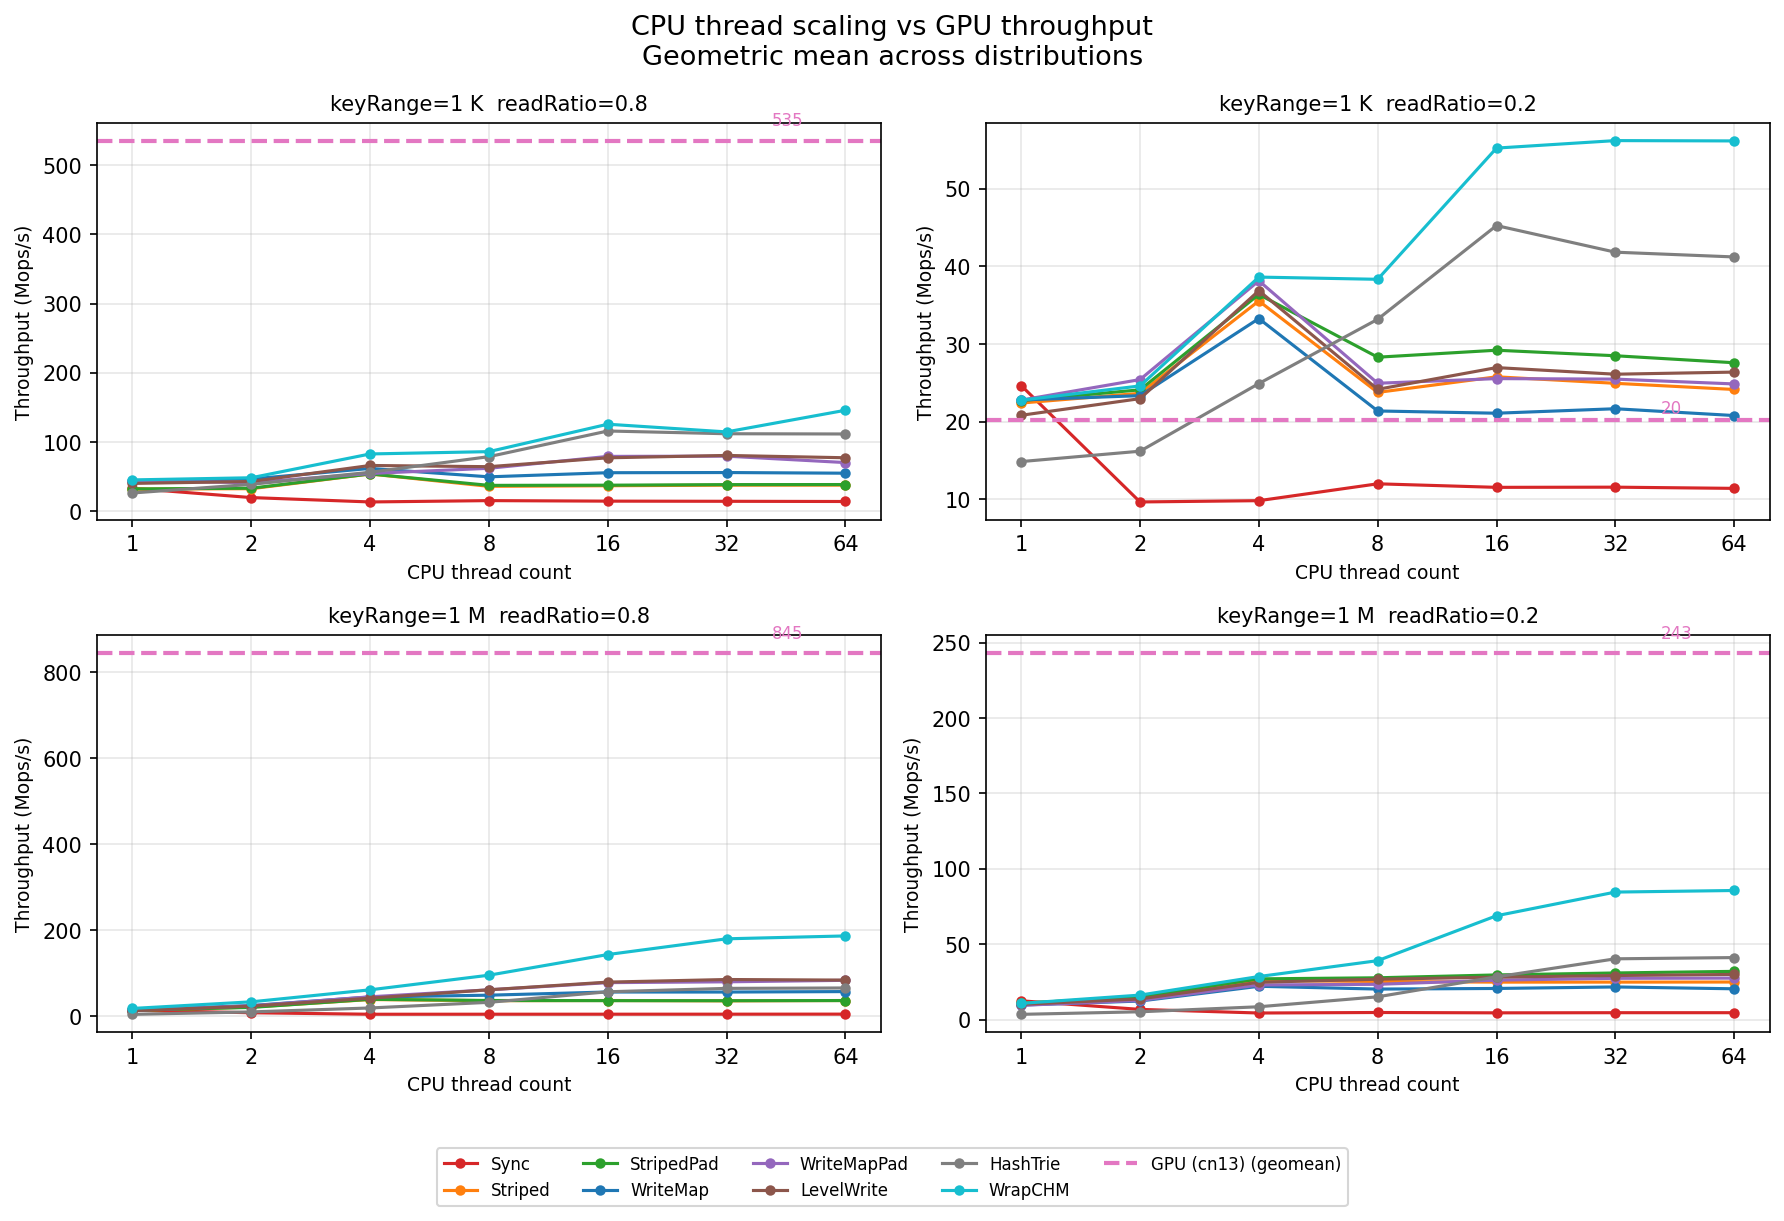
\includegraphics[width=\linewidth]{fig1_cpu_scaling_vs_gpu.png}
  \caption{CPU thread scaling vs.\ GPU throughput (geometric mean across
           distributions). Rows: key range (1\,K / 1\,M). Columns: read
           ratio (0.8 / 0.2). The dashed line marks GPU throughput; CPU
           implementations that cross this line are competitive with the GPU.}
  \label{fig:scaling}
\end{figure}

\subsection{Peak CPU vs.\ GPU Across All Configurations}

Figure~\ref{fig:bar} compares the best CPU implementation
(\texttt{WrapConcurrentHashMap} at 64 threads) with the GPU across all 18
workload configurations. This makes explicit which configurations favour the
GPU and which favour the CPU.

\begin{figure}[h]
  \centering
  \includegraphics[width=\linewidth]{fig2_cpu_peak_vs_gpu.png}
  \caption{Throughput of the best CPU implementation (WrapCHM, 64 threads)
           versus the GPU hash table across all 18 workload configurations.}
  \label{fig:bar}
\end{figure}

\subsection{Read Ratio Sensitivity}

Figure~\ref{fig:readratio} shows how throughput varies with read ratio for
CPU implementations at peak thread count and for the GPU, split by key range.
A steeper positive slope indicates greater benefit from read-heavy workloads.

\begin{figure}[h]
  \centering
  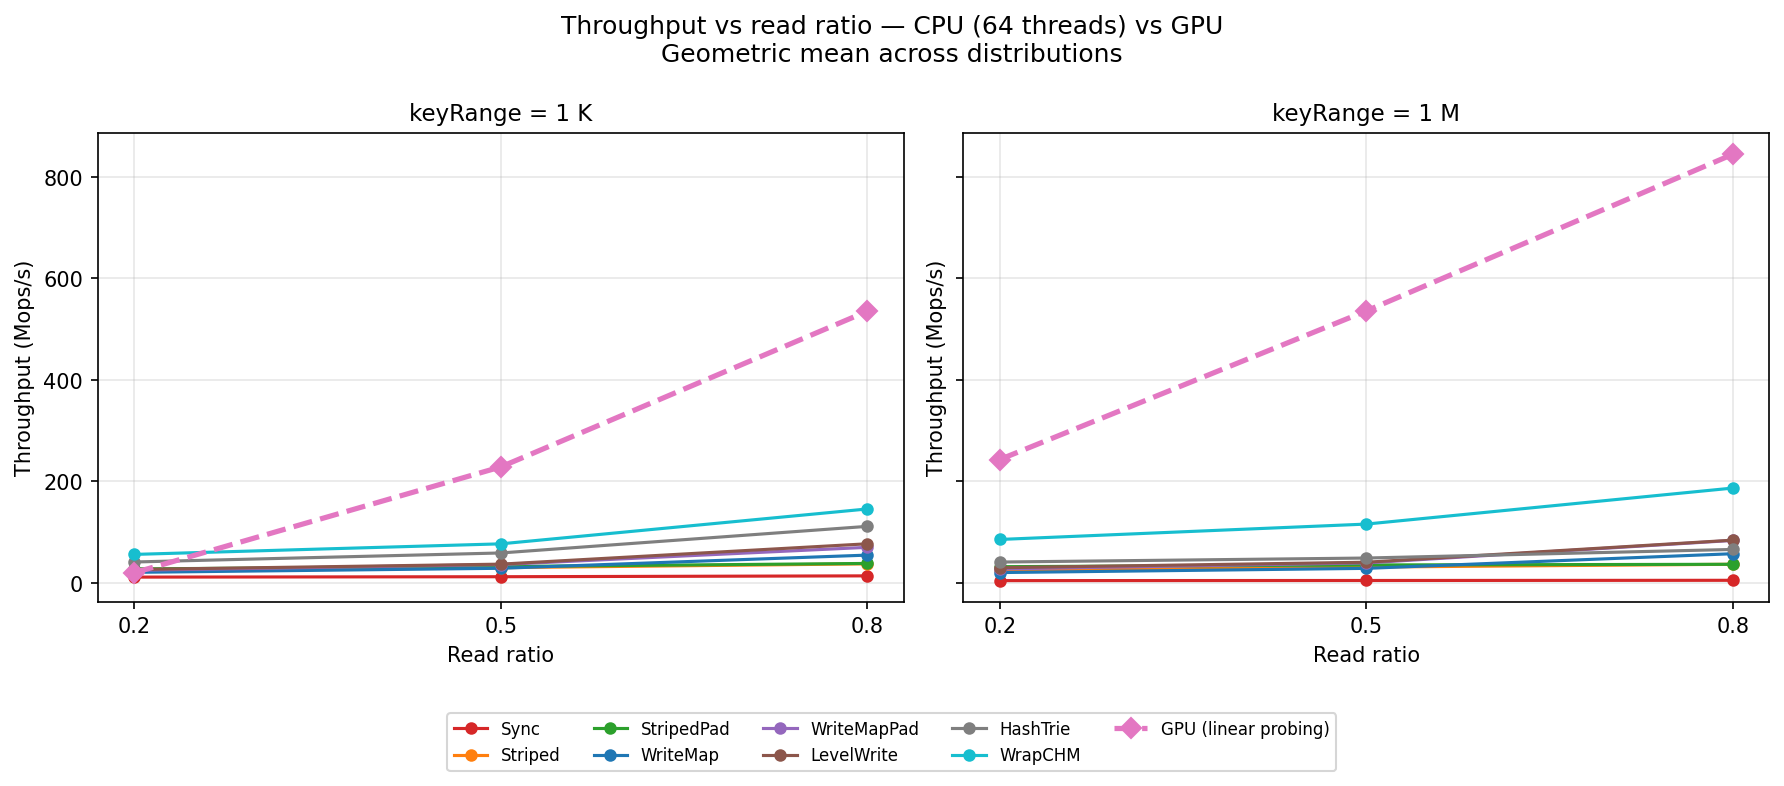
\includegraphics[width=\linewidth]{fig3_read_ratio_sensitivity.png}
  \caption{Throughput vs.\ read ratio at peak thread count (geometric mean
           across distributions). Left: 1\,K keys. Right: 1\,M keys.}
  \label{fig:readratio}
\end{figure}

\subsection{Distribution Sensitivity}

Figure~\ref{fig:dist} shows the percentage throughput change from uniform to
Zipfian-0.99 access at peak thread count, for both CPU implementations and the
GPU. Positive values indicate that skewed access reduces throughput relative to
uniform; negative values indicate it helps.

\begin{figure}[h]
  \centering
  
\includegraphics[width=\linewidth]{fig4_distribution_sensitivity.png}
  \caption{Throughput change from uniform to Zipfian-0.99 at peak thread count,
           per implementation and key range. Positive = skew hurts;
           negative = skew helps.}
  \label{fig:dist}
\end{figure}

% ── 4. Conclusions ────────────────────────────────────────────────────────────
\section{Conclusions}

This project compared the throughput of eight Java concurrent hash table
implementations on a multi-core ARM CPU with a GPU-accelerated open-addressing
hash table across 18 workload configurations.

\textit{[To be completed with actual results.]}

% ── References ───────────────────────────────────────────────────────────────
\bibliographystyle{plain}
\begin{thebibliography}{9}

\bibitem{chen2018}
Z.~Chen et al.,
``Concurrent hash tables on multicore machines,''
\textit{Future Generation Computer Systems}, vol.~82, pp.~127--141, 2018.

\bibitem{sestoft2025}
P.~Sestoft,
``Multicore performance, two case studies,''
Presentation, IT University of Copenhagen, 2025, updated 2025-08-18.

\end{thebibliography}

\end{document}
